\documentclass[10pt,letterpaper]{article}
\usepackage[T1]{fontenc}\usepackage[utf8]{inputenc}\usepackage{mathptmx}
\usepackage[margin=0.68in]{geometry}\usepackage{microtype}\usepackage{booktabs}\usepackage{graphicx}\usepackage{caption}\usepackage{tabularx}\usepackage{ragged2e}
\usepackage[hidelinks]{hyperref}
\captionsetup{font=small,labelfont=bf,justification=RaggedRight,singlelinecheck=false}
\newcolumntype{Y}{>{\RaggedRight\arraybackslash}X}
\setlength{\parindent}{0pt}\setlength{\parskip}{4pt}
\title{\vspace{-18pt}\large Compiling for a device that keeps moving:\\ placement and routing at 78.5 against a 283.5 baseline, and what the compiled circuit is worth at run time}
\author{\normalsize Matthew Stanley Leibel, TrueLoop Compute (NEOTECH Inc.) \quad QSITE 2026 Quantum Coalition, Computational Track}
\date{\normalsize September 2026}
\begin{document}\maketitle\vspace{-16pt}

\textbf{Summary.} Our \texttt{solve()} routes all six benchmarks for a total score of 78.5, 72\% below the provided baseline's 283.5, with every result valid under the track's scorer. Two benchmarks route with zero SWAPs at the minimum possible depth. The second half of the submission asks the question compilation leaves open: a routed circuit is a compile-time object, and what a user receives is its success on a device that drifts after it was characterized. We execute our routed circuits a thousand times on a drifting device model and compare four ways of living with that drift. Free-running loses 14\% of the compiler's promised success on the hardest benchmark; a scheduled recalibration every 200 executions recovers little and dips to 70\% of the promise between visits; a stability contract holding every edge and qubit in-band, from one parallel acquisition per execution, delivers 99\% of the promise for the whole run at 81\,$\mu$s of host time per execution. Scaling the hardware graph to 80,387 channels, the contract's residual stays flat and its cost stays linear, while the dense model a state-reconstruction approach would carry reaches 103\,GB.

\section*{1. The compiler}
\textbf{What the scorer allows.} The routed program must reproduce the original 2Q gate list exactly, in order and orientation; only SWAPs and the initial placement are free; depth is the ASAP critical path over 2Q and SWAP operations; score is SWAPs plus half the depth. So the wins are in the placement, in which qubit moves along which path for each gate, and in SWAPs that do not lengthen the critical path.

\textbf{Placement.} The program's interaction graph is weighted by gate multiplicity with earlier gates weighted more (they are routed first). Simulated annealing over injective placements (swap two logical qubits' physical positions, or move one to a free physical qubit) minimizes the weighted sum of hardware distances.

\textbf{Routing.} Gates are routed strictly in order. While a gate's qubits are not adjacent, the candidate SWAPs are those incident to either qubit that bring them exactly one step closer, which guarantees the minimum $d{-}1$ SWAPs for a gate at distance $d$ and rules out oscillation. Among candidates, the cost is the current gate's distance plus decayed distances of the next 8 gates (SABRE's lookahead) plus a charge for the ASAP layer the SWAP would land on, so SWAPs that ride in an idle slot are preferred over SWAPs that extend the critical path. Four lookahead settings are tried per placement. \textbf{Refinement.} SABRE reverse passes: route forward, route the reversed program from the final layout, and use its final layout as the new initial placement, three times. Then random restarts with the exact scorer in the loop; the returned solution is the best of 120 restarts over three seeds, deterministic.

\begin{table}[h]\caption{Scores by benchmark (lower is better). Baseline is the provided greedy router.}
\small\begin{tabularx}{\textwidth}{Y r r r r r}\toprule
Benchmark & gates & baseline & ours & SWAPs & depth\\\midrule
ghz\_star (star on a max-degree-3 graph) & 7 & 14.0 & 7.0 & 3 & 8\\
chain\_trotter & 9 & 15.0 & 4.5 & 0 & 9\\
ladder\_trotter & 16 & 35.5 & 6.5 & 3 & 7\\
qaoa\_random (12 qubits, 18 random pairs) & 18 & 39.0 & 11.5 & 6 & 11\\
dense\_random (14 qubits, 40 random pairs) & 40 & 122.0 & 46.0 & 33 & 26\\
vqe\_layers (16 wide, 3 repeats): zero SWAPs at the optimal depth 6 & 45 & 58.0 & 3.0 & 0 & 6\\\midrule
Total & & 283.5 & 78.5 & & \\
\bottomrule\end{tabularx}\end{table}

\section*{2. What the compiled circuit is worth at run time}
The compiler's promise for a routed circuit is its success probability on the device as characterized. On real hardware the calibration of every two-qubit gate and every qubit drifts after characterization, which is why teams re-map circuits around bad pairs each morning from the day's fidelity data. We model this directly. Every hardware edge and every qubit is a channel with a coherent angle error that is zero when the compiler characterizes the device and then drifts: a mean-reverting wander of 4\% RMS, half common-mode and half independent, plus a slow non-reverting walk of 0.2\% per execution. A gate's infidelity is a fixed floor (0.6\% two-qubit, 0.05\% single-qubit) plus $\epsilon^2/4$; a SWAP costs three CNOTs; the routed circuit's success is the product over its operations. Four arms on the same drift trajectory:

\begin{itemize}\setlength\itemsep{1pt}
\item \textbf{Compiler's promise}: the characterized device, a constant.
\item \textbf{Free-running}: nobody maintains the device.
\item \textbf{Engineer visit}: a full recalibration every 200 executions (scheduled maintenance, one engineer per site per shift).
\item \textbf{Stability contract}: every channel held in-band. Each execution is preceded by one parallel acquisition of amplified probes on all 43 channels (23 edges, 20 qubits; three-fold rotation probes, 4,000 shots); the readings go to a per-channel controller (TrueLoop v3.1.0) that corrects only above the measured noise floor, learns each channel's slope and sign from its own motion, and applies corrections as scales on the next execution's angles. Nothing is re-compiled.
\end{itemize}

\begin{figure}[t]\centering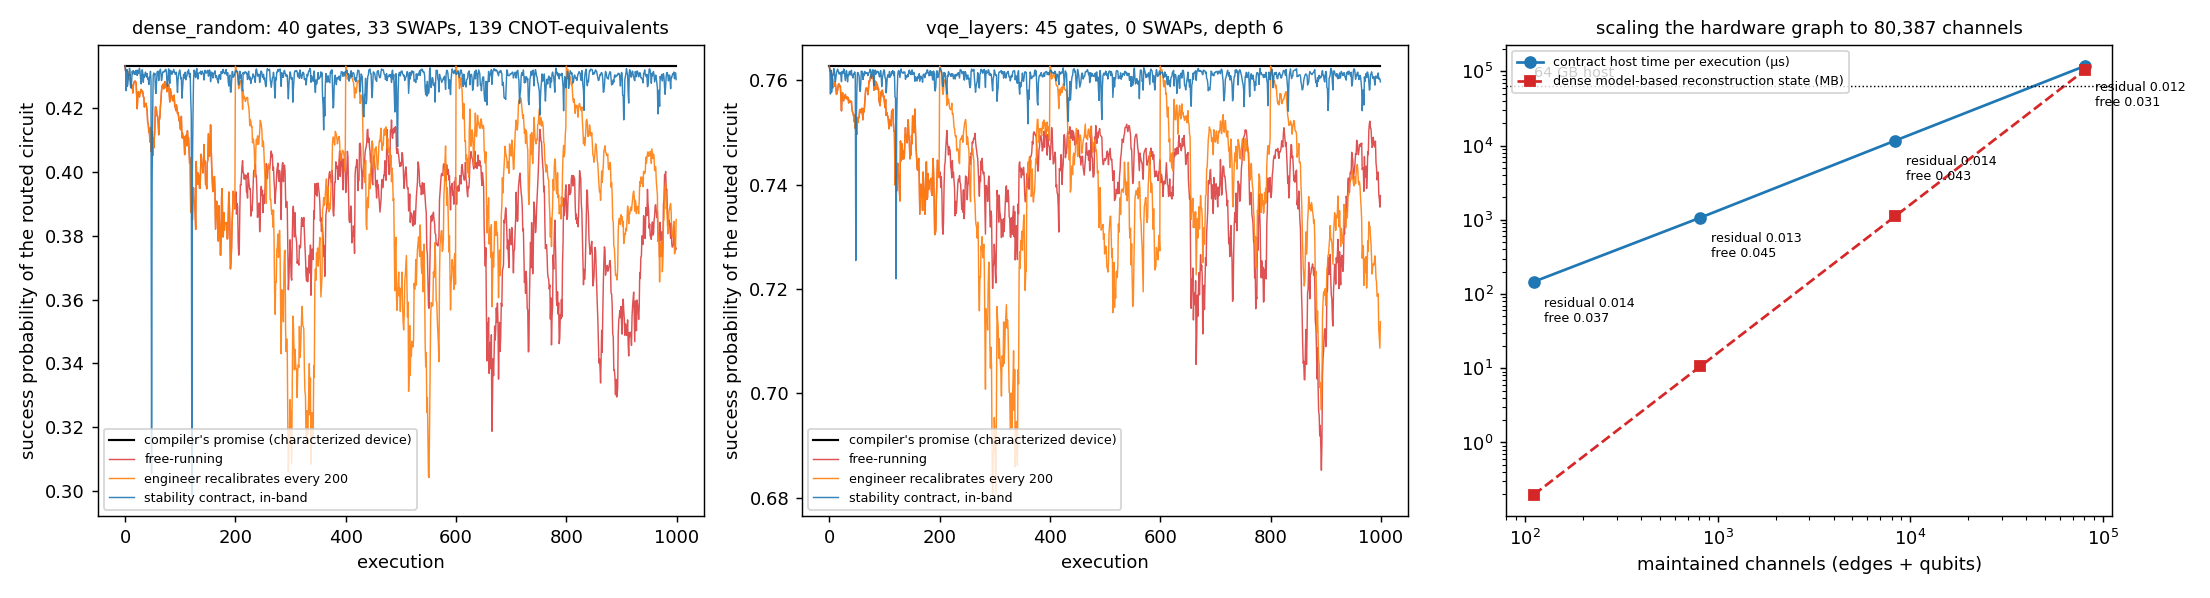
\includegraphics[width=0.82\textwidth]{../figures/runtime_validity.png}
\caption{Left, centre: success probability of two routed circuits over 1,000 executions on the drifting device. Right: host time per execution for the contract on hexagonal-lattice hardware graphs from 111 to 80,387 channels, against the memory a dense model-based reconstruction of the same channels would carry.}\end{figure}

\begin{table}[h]\caption{Run-time success over 1,000 executions (mean, and mean of the last 100).}
\small\begin{tabularx}{\textwidth}{Y r r r r}\toprule
Arm & dense\_random mean & last 100 & vqe\_layers mean & last 100\\\midrule
compiler's promise & 0.433 & 0.433 & 0.763 & 0.763\\
free-running & 0.389 & 0.373 & 0.741 & 0.736\\
engineer recalibrates every 200 & 0.396 (min 0.304) & 0.390 & 0.741 (min 0.681) & 0.731\\
stability contract, 81\,$\mu$s per execution & \textbf{0.429} & \textbf{0.429} & \textbf{0.761} & \textbf{0.760}\\
\bottomrule\end{tabularx}\end{table}

The maintained device delivers 99\% of the compiler's promise on both circuits for the entire run. Free-running delivers 86\% by the end on the dense circuit. The scheduled engineer barely improves on free-running, because a 4\% wander with a fifty-execution correlation time moves faster than any visiting schedule, and each visit only removes the slow walk. This is the mechanism behind ``re-map every morning'': the cost model the compiler used is stale by the time the circuit runs, and maintenance is what keeps it true.

\textbf{Scale.} On hexagonal-lattice graphs from 111 to 80,387 channels (48 to 32,256 qubits), the contract's residual angle error stays at 0.012 to 0.014 against 0.031 to 0.045 free-running, and host time per execution grows linearly at 1.5\,$\mu$s per channel, 118\,ms at 80,387 channels. A model-based alternative that reconstructs the device's state before correcting it carries a dense $n{\times}n$ model: 11\,MB at 815 channels, 1.1\,GB at 8,319, and 103\,GB at 80,387, past what a host can hold, and with setup arithmetic growing as $n^3$. That is why calibration is a scheduled event today and why it cannot stay one at fleet scale: no site can keep engineers on standby for a device with tens of thousands of channels, and no host can reconstruct it. A linear in-band contract is the only one of the three that scales.

\textbf{Limitations.}
The drift model is a simulation with hardware-measured structure, not a measurement on the 20-qubit device; the floors and the 4\% wander are stated assumptions; the probe rung must be an odd multiple of $\pi/2$ with the correction bounds inside its monotone range, which we learned by breaking it; no Stretch Goal A. On a real processor the experiment runs as written: probes are circuits, corrections are angle scales. Code, results, figure, and the maintenance layer's evaluation build are in the package.

\vspace{2pt}\scriptsize\textbf{References.} [1] Quantum Coalition, \emph{QSITE 2026 Computational Track handout and starter kit}, github.com/benmcdonough20/QSITE-2026-QuantumCoalition (hardware graph, benchmarks, scorer, baseline router). [2] G.~Li, Y.~Ding, Y.~Xie, ``Tackling the qubit mapping problem for NISQ-era quantum devices,'' ASPLOS 2019, arXiv:1809.02573: the SABRE lookahead and reverse-pass heuristics adapted here. [3] NetworkX (A.~Hagberg, D.~Schult, P.~Swart, 2008), used by the starter kit and the solver. [4] M.~S.~Leibel, ``A Stability Contract for Scalable Hybrid Computing: Minimal Sufficient Control of Component-Observable Hardware,'' Preprints 202609.1101 (2026), doi:10.20944/preprints202609.1101.v1, under review at IEEE Trans.\ Computers: the maintenance layer's method and bounds; the evaluation build of TrueLoop v3.1.0 (NEOTECH Inc.) is included. [5] NumPy, Matplotlib.

\end{document}
